\listfiles
\documentclass{article}

\usepackage{amsmath}
\usepackage{amssymb}
\usepackage{mathtools}
\usepackage{listings}
\usepackage{hyperref}

\DeclarePairedDelimiter\floor{\lfloor}{\rfloor}
\DeclarePairedDelimiter\ceil{\lceil}{\rceil}
\DeclareMathOperator{\cl}{cl}
\DeclareMathOperator{\E}{E}
\def\Z{\mathbb{Z}}
\def\N{\mathbb{N}}
\def\R{\mathbb{R}}
\def\Q{\mathbb{Q}}
\def\K{\mathbb{K}}
\def\T{\mathbb{T}}
\def\B{\mathcal{B}}
\def\XX{\mathfrak{X}}
\def\YY{\mathfrak{Y}}
\def\AA{\mathfrak{A}}
\def\ZZ{\mathfrak{Z}}
\def\BB{\mathcal{B}}
\def\UU{\mathcal{U}}
\def\MM{\mathcal{M}}
\def\M{\mathfrak{M}}
\def\l{\lambda}
\def\L{\Lambda}
\def\<{\langle}
\def\>{\rangle}
\def\f12{\frac{1}{2}}
\def\inv{{-1}}

\usepackage[a4paper,margin=1in]{geometry}

\setlength{\parindent}{0cm}
\setlength{\parskip}{1em}

\title{HW 3}
\date{}

\begin{document}
\maketitle

\section*{1a.}

It suffices to show that each cycle $(a_1, a_2, \ldots a_k)$ is generated by 2-cycles. This is true because $(a_1, a_2, \ldots a_k) = (a_1, a_2)(a_2, a_3)\ldots(a_{k-1}, a_k)$, which we can see by having it operate on an arbitrary $a_j$ from right to left. If $j \ne k$, the first 2-cycle that does not fix its argument is $(a_j, a_{j+1})$ which sends it to $a_{j+1}$. Now the next 2-cycle is $(a_{j-1}, a_j)$ which fixes $a_{j+1}$; every other 2-cycle also fixes it since the indices are decreasing. If $j = k$, each 2-cycle reduces the index of $j$ by one, and we end up with $a_1$.

\section*{1b.}

The identity has 0 inversions and is even.

A transposition has an odd number of inversions. Proof: count the number of inversions modulo 2. Call a pair of indices a candidate inversion if its elements are strictly increasing; the inversions are in bijection with candidate inversions which are mapped by $\sigma$ to a decreasing tuple. Let the transposition be $(a, b)$ with $a < b$. If $[i, j]$ is a candidate inversion, suppose $\{i, j\}$ is disjoint with $\{a, b\}$, then $[i, j]$ is mapped to $[\sigma(i), \sigma(j)] = [i, j]$ so $[i, j]$ does not correspond to an inversion. Hence it suffices to consider candidate inversions where at least one of the indices is $a$ or $b$.

First consider the candidate inversions where exactly one of the incides is $a$ or $b$. If the other index is $< a$ then the pair is $[i, a]$ which is mapped to $[i, b]$, so the candidate does not correspond to an inversion since $i < b$. Similarly if the other index is $> b$, we contribute 0 to the sum.

Consider the candidate inversions where exactly one of the indices is $a$ or $b$ and the other index is between $a$ and $b$. For every $k$ where $a < k < b$, we have the two distinct candidate inversions $[a, k]$ and $[k, b]$ which fall in this category, and they are mapped to $[b, k]$ and $[k, a]$. These correspond to 2 inversions and contribute 0 to the sum.

We are left with the candidate inversions $[a, b]$; this is mapped to $[b, a]$ hence it corresponds to an inversion.

\section*{1c.}

The proof is similar to 1b; we want to compare the number of inversions in the list $[\sigma(1), \sigma(2), \ldots \sigma(n)]$ before and after swapping two elements. WLOG those two elements are $\sigma(i)$ and $\sigma(j)$ for some $i < j$. Among the candidate inversions $[i', j']$ if $\{i', j'\}$ is disjoint from $T = \{\sigma(i), \sigma(j)\}$ then it is unaffected by the transposition; of those where exactly one of them lies in $T$, they are paired up because every $k$ such that $i < k < j$ leads to two candidate inversions, and the pair either causes the number of inversions to increase by two (if $\sigma(i) < \sigma(j)$) or decrease by two (otherwise); and there is one candidate whose elements are exactly $T$, where the number of inversions increases or decreases by one.

\section*{1d.}

Every permutation can be written as a product of transpositions (by 1a). By 1b and 1c, an even permutation can be written as a product of an even number of transpositions, and an odd permutation can be written as a product of an odd number of transpositions.

Let $Q, R$ be odd permutations and consider $P = QR$. We can write $Q = q_1q_2 \ldots q_k$ ($k$ odd) and $R = r_1r_2 \ldots r_l$ ($l$ odd), means we can write $P = q_1q_2 \ldots q_kr_1r_2 \ldots r_l$ which has $k + l$ transpositions, hence $P$ is even by 1b and 1c.

The proofs for the other 3 cases of the parity of $Q, R$ are identical.

\section*{Section 1.4}

\section*{7}

It suffices to show that the number of singular matrices is $p^3 + p^2 - p$, since the total number of matrices is $p^4$. The singular matrices either have first row equal to 0 or not. Of the matrices with first row 0, there are $p^2$ choices for the second row (no restrictions). There are $p^2 - 1$ nonzero first rows, and each of them corresponds to $p$ singular matrices (one for each multiple of the first row, since there are $p$ distinct multiples). Hence the total number is $p^2 + p(p^2 - 1) = p^3 + p^2 - p$.

\section*{Section 1.6}

Lemma: if $\phi: G \to H$ is a group isomoprhism, then the inverse of $\phi$ (taken as a set function, which exists because $\phi$ is bijective) is a group isomoprhism.

Proof: it is required to show that $\phi^\inv(xy) = \phi^\inv(x)\phi^\inv(y)$ for all $x, y \in H$. We have $\phi(\phi^\inv(xy)) = \phi(\phi^\inv(x)\phi^\inv(y))$ because the LHS is $xy$ and the RHS is $\phi(\phi^\inv(x)\phi^\inv(y)) = (\phi(\phi^\inv(x))) (\phi(\phi^\inv(y))) = xy$ where the first equality holds because $\phi$ is a group homomorphism. The result follows because $\phi$ is injective.

\section*{1}

We prove part a by induction on $n$. We will use $n=1$ as the base case, which is trivial. For the inductive step, we have $\phi(x^{n+1}) = \phi(x^n x) = \phi(x^n) \phi(x) = \phi(x)^n \phi(x) = \phi(x)^{n+1}$.

Additionally we will prove that $\phi(e) = e$. Let $\phi(e) = x$, then $x = \phi(e) = \phi(ee) = x^2$; cancelling, we have $x = e$.

For part b, it is required to prove that $\phi(x^\inv) = \phi(x)^\inv$, equivalently $\phi(x) \phi(x^\inv) = e$. This follows because $\phi(x) \phi(x^\inv) = \phi(x x^\inv) = \phi(e) = e$.

The extension to $\Z$ then follows by applying part (a) to the element $x^\inv$, since $\phi(x^{-n}) = \phi((x^\inv)^n) = (\phi(x)^\inv)^n = \phi(x)^{-n}$.

\section*{2}

Let $n = ord(x)$. Then $\phi(x)^n = \phi(x^n) = \phi(e) = e$, hence $ord(\phi(x)) \le n$. Similarly, by the lemma, $ord(\phi(x)) \ge n$, hence $ord(\phi(x)) = n$.

The trivial homomorphism $\phi: G \to H$ that sends every element to the identity shows that this is not true for just homomorphisms, since there exists groups with different number of elements of order 4 (e.g. $Z_4$ has two such element and the quaternion group has 6)

\section*{3}

Let $H$ be abelian. Then for all $x, y \in G$ we have $xy = \phi(\phi^\inv(x) \phi^\inv(y)) = \phi(\phi^\inv(y) \phi^\inv(x)) = yx$. The proof for when $G$ is abelian is the same proof applied to the isomoprhism $\phi^\inv$.

For a sujective homomorphism $\phi: G \to H$, if $G$ is abelian then $H$ is abelian. Let $h_1, h_2 \in H$. We know that there are elements $g_1, g_2$ satisfying $g_1 = h_1, g_2 = h_2$, and applying $\phi$ to the identity $g_1 g_2 = g_2 g_1$ leads to $h_1 h_2 = h_2 h_1$.

\section*{6}

$\Z$ is generated by $1$. If $\Q$ is isomorphic to $\Z$ then $\phi(1)$ also generates $\Q$ since any element $n \in \Z$ can be mapped to $n\phi(i)$. Let $q = \phi(1)$.

It is easy to see that $q \ne 0$. Then the element $\frac{q}{2}$ is not in $\Q$ because the equation $nq = \frac{q}{2}$ has no integer solutions in $n$.

\section*{14}

We will first prove exercise 26. First, $e \in H$; since $H$ is nonempty, take some $x \in H$, we have $e = x x^\inv$ which is a product of two elements in $H$. The fact that the group operation in $H$ is associative and that $e$ is an identity under that operation follow by considering those elements as elements of $G$.

It remains to show that $\ker \phi$ is closed under the group operation and under inverse. First, suppose $x, y \in \ker G$, which means $\phi(x) = \phi(y) = e$. Then $\phi(xy) = \phi(x) \phi(y) = e^2 = e$ hence $\phi(xy) \in \ker G$. Secondly, $\phi(x^\inv) = \phi(x)^\inv = e^\inv = e$, hence $x^\inv \in \ker G$.

$\phi$ is injective $\iff \ker G = \{e\}$. $\implies$: let $x \in \ker G$, that is $\phi(x) = e = \phi(e)$; applying the injectivity of $\phi$ to the equation $\phi(x) = \phi(e)$ yields $x = e$. $\impliedby$: suppose $\phi(x) = \phi(y)$ for some $x, y \in G$. We can rewrite this as $e = \phi(x)^\inv\phi(y) = \phi(x^\inv y)$, hence $x^\inv y \in \ker G$, hence $x^\inv y = e$, hence $x = y$.

\section*{17}

Let $\phi$ be the map. Suppose $G$ is abelian. Then for all $x, y \in G$ we have $\phi(xy) = (xy)^\inv = y^\inv x^\inv = x^\inv y^\inv = \phi(x) \phi(y)$ where the 3rd equation follows because $G$ is abelian.

Conversely suppose $\phi$ is a homomorphism and let $x, y \in G$. Then $xy = (y^\inv x^\inv)^\inv = \phi(y^\inv x^\inv) = \phi(y^\inv) \phi(x^\inv) = yx$

\section*{25a}

Let $M$ be the matrix in the question. Since the question presupposes that a rotation is a linear transformation, it suffices to show that $M$ is a rotation on any basis of $\R^2$; we will take $\{[-1, 0], [1, 0]\}$ which $M$ maps to $\{[-\cos\theta, -\sin\theta], [-\sin\theta, \cos\theta]\}$. A geometric proof is attached.

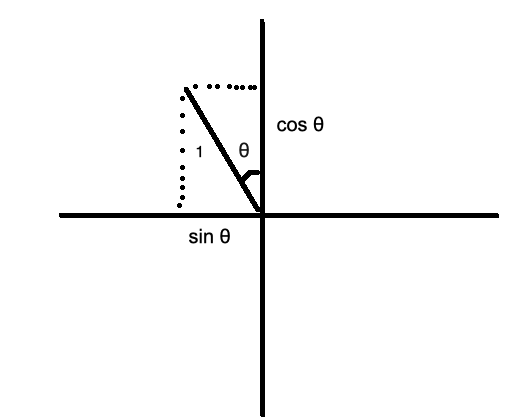
\includegraphics[scale=0.65]{basis1.png}

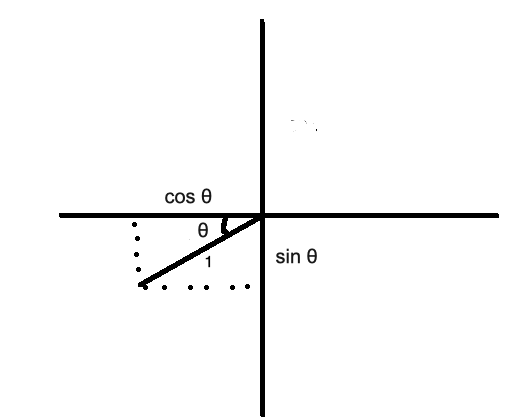
\includegraphics[scale=0.65]{basis2.png}

\section*{25b}

We have to show that the generator relations are satisfied.

$\phi(r)^n = I$; since $\phi(r)$ is a ccw rotation by $\theta$, $\phi(r)^n$ is a ccw rotation by $n\theta = 2\pi$, which is the identity map.

$\phi(s)^2 = I$; this is a simple computation.

The relation $\phi(r)\phi(s)\phi(r) = \phi(s)$ can be verified by wolfram alpha \url{https://www.wolframalpha.com/input?i=%5B%5Bcos+x%2C+-sin+x%5D%2C+%5Bsin+x%2C+cos+x%5D%5D+%5B%5B0%2C+1%5D%2C+%5B1%2C+0%5D%5D+%5B%5Bcos+x%2C+-sin+x%5D%2C+%5Bsin+x%2C+cos+x%5D%5D}

\section*{25c}

It suffices to show that the $2n$ elements $\phi(r)^i \phi(s)^j$ for $i \in [0, n), j \in \{0, 1\}$ are distinct matrices. First, if two such elements have different $j$, they have different determinants, since $\det \phi(r) = 1, \det \phi(s) = -1$. Next, we will prove that all the $\{\phi(r)^i\}_i$ are distinct, which is sufficient since $\phi(s)$ is injective when considered as a linear map. If we consider the first column of each of those matrices and map the column $[a, b]$ to the complex number $a + bi$ the $\{\phi(r)^i\}_i$ are mapped to $[0, z, z^2 \ldots z^{n-1}]$ where $z = e^{i\theta}$. These are the $n$ (distinct) roots of unity since $\theta = 2\pi/n$, hence the first columns (and hence matrices) are distinct.


\end{document}
